\documentclass[1p]{elsarticle_modified}
%\bibliographystyle{elsarticle-num}

%\usepackage[colorlinks]{hyperref}
%\usepackage{abbrmath_seonhwa} %\Abb, \Ascr, \Acal ,\Abf, \Afrak
\usepackage{amsfonts}
\usepackage{amssymb}
\usepackage{amsmath}
\usepackage{amsthm}
\usepackage{scalefnt}
\usepackage{amsbsy}
\usepackage{kotex}
\usepackage{caption}
\usepackage{subfig}
\usepackage{color}
\usepackage{graphicx}
\usepackage{xcolor} %% white, black, red, green, blue, cyan, magenta, yellow
\usepackage{float}
\usepackage{setspace}
\usepackage{hyperref}

\usepackage{tikz}
\usetikzlibrary{arrows}

\usepackage{multirow}
\usepackage{array} % fixed length table
\usepackage{hhline}

%%%%%%%%%%%%%%%%%%%%%
\makeatletter
\renewcommand*\env@matrix[1][\arraystretch]{%
	\edef\arraystretch{#1}%
	\hskip -\arraycolsep
	\let\@ifnextchar\new@ifnextchar
	\array{*\c@MaxMatrixCols c}}
\makeatother %https://tex.stackexchange.com/questions/14071/how-can-i-increase-the-line-spacing-in-a-matrix
%%%%%%%%%%%%%%%

\usepackage[normalem]{ulem}

\newcommand{\msout}[1]{\ifmmode\text{\sout{\ensuremath{#1}}}\else\sout{#1}\fi}
%SOURCE: \msout is \stkout macro in https://tex.stackexchange.com/questions/20609/strikeout-in-math-mode

\newcommand{\cancel}[1]{
	\ifmmode
	{\color{red}\msout{#1}}
	\else
	{\color{red}\sout{#1}}
	\fi
}

\newcommand{\add}[1]{
	{\color{blue}\uwave{#1}}
}

\newcommand{\replace}[2]{
	\ifmmode
	{\color{red}\msout{#1}}{\color{blue}\uwave{#2}}
	\else
	{\color{red}\sout{#1}}{\color{blue}\uwave{#2}}
	\fi
}

\newcommand{\Sol}{\mathcal{S}} %segment
\newcommand{\D}{D} %diagram
\newcommand{\A}{\mathcal{A}} %arc


%%%%%%%%%%%%%%%%%%%%%%%%%%%%%5 test

\def\sl{\operatorname{\textup{SL}}(2,\Cbb)}
\def\psl{\operatorname{\textup{PSL}}(2,\Cbb)}
\def\quan{\mkern 1mu \triangleright \mkern 1mu}

\theoremstyle{definition}
\newtheorem{thm}{Theorem}[section]
\newtheorem{prop}[thm]{Proposition}
\newtheorem{lem}[thm]{Lemma}
\newtheorem{ques}[thm]{Question}
\newtheorem{cor}[thm]{Corollary}
\newtheorem{defn}[thm]{Definition}
\newtheorem{exam}[thm]{Example}
\newtheorem{rmk}[thm]{Remark}
\newtheorem{alg}[thm]{Algorithm}

\newcommand{\I}{\sqrt{-1}}
\begin{document}

%\begin{frontmatter}
%
%\title{Boundary parabolic representations of knots up to 8 crossings}
%
%%% Group authors per affiliation:
%\author{Yunhi Cho} 
%\address{Department of Mathematics, University of Seoul, Seoul, Korea}
%\ead{yhcho@uos.ac.kr}
%
%
%\author{Seonhwa Kim} %\fnref{s_kim}}
%\address{Center for Geometry and Physics, Institute for Basic Science, Pohang, 37673, Korea}
%\ead{ryeona17@ibs.re.kr}
%
%\author{Hyuk Kim}
%\address{Department of Mathematical Sciences, Seoul National University, Seoul 08826, Korea}
%\ead{hyukkim@snu.ac.kr}
%
%\author{Seokbeom Yoon}
%\address{Department of Mathematical Sciences, Seoul National University, Seoul, 08826,  Korea}
%\ead{sbyoon15@snu.ac.kr}
%
%\begin{abstract}
%We find all boundary parabolic representation of knots up to 8 crossings.
%
%\end{abstract}
%\begin{keyword}
%    \MSC[2010] 57M25 
%\end{keyword}
%
%\end{frontmatter}

%\linenumbers
%\tableofcontents
%
\newcommand\colored[1]{\textcolor{white}{\rule[-0.35ex]{0.8em}{1.4ex}}\kern-0.8em\color{red} #1}%
%\newcommand\colored[1]{\textcolor{white}{ #1}\kern-2.17ex	\textcolor{white}{ #1}\kern-1.81ex	\textcolor{white}{ #1}\kern-2.15ex\color{red}#1	}

{\Large $\underline{12a_{0368}~(K12a_{0368})}$}

\setlength{\tabcolsep}{10pt}
\renewcommand{\arraystretch}{1.6}
\vspace{1cm}\begin{tabular}{m{100pt}>{\centering\arraybackslash}m{274pt}}
\multirow{5}{120pt}{
	\centering
	\includegraphics[width=112pt]{../../../GIT/diagram.site/Diagrams/png/1169_12a_0368.png}\\
\ \ \ A knot diagram\footnotemark}&
\allowdisplaybreaks
\textbf{Linearized knot diagam} \\
\cline{2-2}
 &
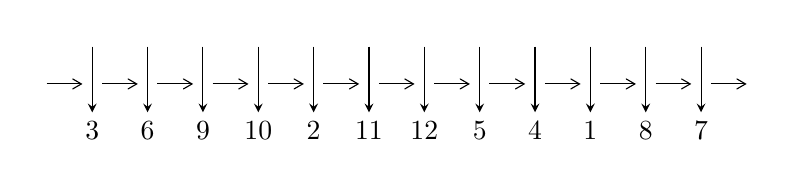
\begin{tikzpicture}[x=20pt, y=17pt]
	% nodes
	\node (C0) at (0, 0) {};
	\node (C1) at (1, 0) {};
	\node (C1U) at (1, +1) {};
	\node (C1D) at (1, -1) {3};

	\node (C2) at (2, 0) {};
	\node (C2U) at (2, +1) {};
	\node (C2D) at (2, -1) {6};

	\node (C3) at (3, 0) {};
	\node (C3U) at (3, +1) {};
	\node (C3D) at (3, -1) {9};

	\node (C4) at (4, 0) {};
	\node (C4U) at (4, +1) {};
	\node (C4D) at (4, -1) {10};

	\node (C5) at (5, 0) {};
	\node (C5U) at (5, +1) {};
	\node (C5D) at (5, -1) {2};

	\node (C6) at (6, 0) {};
	\node (C6U) at (6, +1) {};
	\node (C6D) at (6, -1) {11};

	\node (C7) at (7, 0) {};
	\node (C7U) at (7, +1) {};
	\node (C7D) at (7, -1) {12};

	\node (C8) at (8, 0) {};
	\node (C8U) at (8, +1) {};
	\node (C8D) at (8, -1) {5};

	\node (C9) at (9, 0) {};
	\node (C9U) at (9, +1) {};
	\node (C9D) at (9, -1) {4};

	\node (C10) at (10, 0) {};
	\node (C10U) at (10, +1) {};
	\node (C10D) at (10, -1) {1};

	\node (C11) at (11, 0) {};
	\node (C11U) at (11, +1) {};
	\node (C11D) at (11, -1) {8};

	\node (C12) at (12, 0) {};
	\node (C12U) at (12, +1) {};
	\node (C12D) at (12, -1) {7};
	\node (C13) at (13, 0) {};

	% arrows
	\draw[->,>={angle 60}]
	(C0) edge (C1) (C1) edge (C2) (C2) edge (C3) (C3) edge (C4) (C4) edge (C5) (C5) edge (C6) (C6) edge (C7) (C7) edge (C8) (C8) edge (C9) (C9) edge (C10) (C10) edge (C11) (C11) edge (C12) (C12) edge (C13) ;	\draw[->,>=stealth]
	(C1U) edge (C1D) (C2U) edge (C2D) (C3U) edge (C3D) (C4U) edge (C4D) (C5U) edge (C5D) (C6U) edge (C6D) (C7U) edge (C7D) (C8U) edge (C8D) (C9U) edge (C9D) (C10U) edge (C10D) (C11U) edge (C11D) (C12U) edge (C12D) ;
	\end{tikzpicture} \\
\hhline{~~} \\& 
\textbf{Solving Sequence} \\ \cline{2-2} 
 &
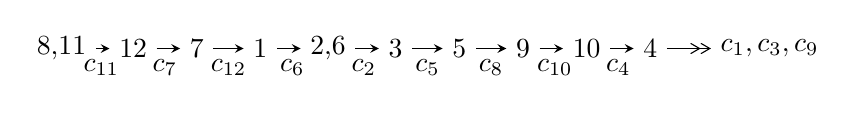
\begin{tikzpicture}[x=23pt, y=7pt]
	% node
	\node (A0) at (-1/8, 0) {8,11};
	\node (A1) at (1, 0) {12};
	\node (A2) at (2, 0) {7};
	\node (A3) at (3, 0) {1};
	\node (A4) at (65/16, 0) {2,6};
	\node (A5) at (41/8, 0) {3};
	\node (A6) at (49/8, 0) {5};
	\node (A7) at (57/8, 0) {9};
	\node (A8) at (65/8, 0) {10};
	\node (A9) at (73/8, 0) {4};
	\node (C1) at (1/2, -1) {$c_{11}$};
	\node (C2) at (3/2, -1) {$c_{7}$};
	\node (C3) at (5/2, -1) {$c_{12}$};
	\node (C4) at (7/2, -1) {$c_{6}$};
	\node (C5) at (37/8, -1) {$c_{2}$};
	\node (C6) at (45/8, -1) {$c_{5}$};
	\node (C7) at (53/8, -1) {$c_{8}$};
	\node (C8) at (61/8, -1) {$c_{10}$};
	\node (C9) at (69/8, -1) {$c_{4}$};
	\node (A10) at (11, 0) {$c_{1},c_{3},c_{9}$};

	% edge
	\draw[->,>=stealth]	
	(A0) edge (A1) (A1) edge (A2) (A2) edge (A3) (A3) edge (A4) (A4) edge (A5) (A5) edge (A6) (A6) edge (A7) (A7) edge (A8) (A8) edge (A9) ;
	\draw[->>,>={angle 60}]	
	(A9) edge (A10);
\end{tikzpicture} \\ 

\end{tabular} \\

\footnotetext{
The image of knot diagram is generated by the software ``\textbf{Draw programme}" developed by Andrew Bartholomew(\url{http://www.layer8.co.uk/maths/draw/index.htm\#Running-draw}), where we modified some parts for our purpose(\url{https://github.com/CATsTAILs/LinksPainter}).
}\phantom \\ \newline 
\centering \textbf{Ideals for irreducible components\footnotemark of $X_{\text{par}}$} 
 
\begin{align*}
I^u_{1}&=\langle 
3.30973\times10^{28} u^{91}-8.40338\times10^{28} u^{90}+\cdots+5.98098\times10^{28} b+1.59798\times10^{28},\\
\phantom{I^u_{1}}&\phantom{= \langle  }-2.69784\times10^{28} u^{91}+1.86728\times10^{28} u^{90}+\cdots+5.98098\times10^{28} a-7.90169\times10^{28},\;u^{92}-2 u^{91}+\cdots+4 u-1\rangle \\
I^u_{2}&=\langle 
- a u- u^2+b+u-1,\;-2 u^2 a+a^2-3 u^2-2 a+u-4,\;u^3- u^2+2 u-1\rangle \\
I^u_{3}&=\langle 
-2 u^2+b-2 u-2,\;- u^2+a-1,\;u^3+u^2+2 u+1\rangle \\
\\
\end{align*}
\raggedright * 3 irreducible components of $\dim_{\mathbb{C}}=0$, with total 101 representations.\\
\footnotetext{All coefficients of polynomials are rational numbers. But the coefficients are sometimes approximated in decimal forms when there is not enough margin.}
\newpage
\renewcommand{\arraystretch}{1}
\centering \section*{I. $I^u_{1}= \langle 3.31\times10^{28} u^{91}-8.40\times10^{28} u^{90}+\cdots+5.98\times10^{28} b+1.60\times10^{28},\;-2.70\times10^{28} u^{91}+1.87\times10^{28} u^{90}+\cdots+5.98\times10^{28} a-7.90\times10^{28},\;u^{92}-2 u^{91}+\cdots+4 u-1 \rangle$}
\flushleft \textbf{(i) Arc colorings}\\
\begin{tabular}{m{7pt} m{180pt} m{7pt} m{180pt} }
\flushright $a_{8}=$&$\begin{pmatrix}0\\u\end{pmatrix}$ \\
\flushright $a_{11}=$&$\begin{pmatrix}1\\0\end{pmatrix}$ \\
\flushright $a_{12}=$&$\begin{pmatrix}1\\u^2\end{pmatrix}$ \\
\flushright $a_{7}=$&$\begin{pmatrix}u\\u^3+u\end{pmatrix}$ \\
\flushright $a_{1}=$&$\begin{pmatrix}u^2+1\\u^4+2 u^2\end{pmatrix}$ \\
\flushright $a_{2}=$&$\begin{pmatrix}0.451070 u^{91}-0.312203 u^{90}+\cdots-7.08977 u+1.32114\\-0.553376 u^{91}+1.40502 u^{90}+\cdots+1.50461 u-0.267177\end{pmatrix}$ \\
\flushright $a_{6}=$&$\begin{pmatrix}u^3+2 u\\u^3+u\end{pmatrix}$ \\
\flushright $a_{3}=$&$\begin{pmatrix}0.735415 u^{91}-0.771047 u^{90}+\cdots-8.70172 u+2.30497\\-0.222428 u^{91}+0.315787 u^{90}+\cdots-0.399025 u+0.493332\end{pmatrix}$ \\
\flushright $a_{5}=$&$\begin{pmatrix}0.362177 u^{91}-0.986787 u^{90}+\cdots+4.35986 u+1.44942\\0.858220 u^{91}-2.63949 u^{90}+\cdots-1.81332 u+0.982411\end{pmatrix}$ \\
\flushright $a_{9}=$&$\begin{pmatrix}-0.918301 u^{91}+2.21912 u^{90}+\cdots-3.90930 u-1.54472\\-0.0236999 u^{91}+0.263544 u^{90}+\cdots+0.339475 u-0.202110\end{pmatrix}$ \\
\flushright $a_{10}=$&$\begin{pmatrix}- u^6-3 u^4-2 u^2+1\\- u^8-4 u^6-4 u^4\end{pmatrix}$ \\
\flushright $a_{4}=$&$\begin{pmatrix}1.29625 u^{91}-2.48311 u^{90}+\cdots+0.388481 u+2.80304\\0.918260 u^{91}-2.71085 u^{90}+\cdots-2.13551 u+1.23180\end{pmatrix}$\\&\end{tabular}
\flushleft \textbf{(ii) Obstruction class $= -1$}\\~\\
\flushleft \textbf{(iii) Cusp Shapes $= -1.75950 u^{91}+3.08333 u^{90}+\cdots-2.35105 u-16.2139$}\\~\\
\newpage\renewcommand{\arraystretch}{1}
\flushleft \textbf{(iv) u-Polynomials at the component}\newline \\
\begin{tabular}{m{50pt}|m{274pt}}
Crossings & \hspace{64pt}u-Polynomials at each crossing \\
\hline $$\begin{aligned}c_{1}\end{aligned}$$&$\begin{aligned}
&u^{92}+46 u^{91}+\cdots+1255 u+49
\end{aligned}$\\
\hline $$\begin{aligned}c_{2},c_{5}\end{aligned}$$&$\begin{aligned}
&u^{92}+4 u^{91}+\cdots-67 u-7
\end{aligned}$\\
\hline $$\begin{aligned}c_{3},c_{4},c_{9}\end{aligned}$$&$\begin{aligned}
&u^{92}- u^{91}+\cdots-24 u-8
\end{aligned}$\\
\hline $$\begin{aligned}c_{6}\end{aligned}$$&$\begin{aligned}
&u^{92}-2 u^{91}+\cdots-312 u-29
\end{aligned}$\\
\hline $$\begin{aligned}c_{7},c_{11},c_{12}\end{aligned}$$&$\begin{aligned}
&u^{92}+2 u^{91}+\cdots-4 u-1
\end{aligned}$\\
\hline $$\begin{aligned}c_{8}\end{aligned}$$&$\begin{aligned}
&u^{92}+3 u^{91}+\cdots+49864 u+10856
\end{aligned}$\\
\hline $$\begin{aligned}c_{10}\end{aligned}$$&$\begin{aligned}
&u^{92}-20 u^{91}+\cdots-103152 u+12161
\end{aligned}$\\
\hline
\end{tabular}\\~\\
\newpage\renewcommand{\arraystretch}{1}
\flushleft \textbf{(v) Riley Polynomials at the component}\newline \\
\begin{tabular}{m{50pt}|m{274pt}}
Crossings & \hspace{64pt}Riley Polynomials at each crossing \\
\hline $$\begin{aligned}c_{1}\end{aligned}$$&$\begin{aligned}
&y^{92}+10 y^{91}+\cdots-468507 y+2401
\end{aligned}$\\
\hline $$\begin{aligned}c_{2},c_{5}\end{aligned}$$&$\begin{aligned}
&y^{92}-46 y^{91}+\cdots-1255 y+49
\end{aligned}$\\
\hline $$\begin{aligned}c_{3},c_{4},c_{9}\end{aligned}$$&$\begin{aligned}
&y^{92}-85 y^{91}+\cdots+448 y+64
\end{aligned}$\\
\hline $$\begin{aligned}c_{6}\end{aligned}$$&$\begin{aligned}
&y^{92}+4 y^{91}+\cdots+28748 y+841
\end{aligned}$\\
\hline $$\begin{aligned}c_{7},c_{11},c_{12}\end{aligned}$$&$\begin{aligned}
&y^{92}+84 y^{91}+\cdots-16 y+1
\end{aligned}$\\
\hline $$\begin{aligned}c_{8}\end{aligned}$$&$\begin{aligned}
&y^{92}- y^{91}+\cdots-514447808 y+117852736
\end{aligned}$\\
\hline $$\begin{aligned}c_{10}\end{aligned}$$&$\begin{aligned}
&y^{92}+28 y^{91}+\cdots-3573140208 y+147889921
\end{aligned}$\\
\hline
\end{tabular}\\~\\
\newpage\flushleft \textbf{(vi) Complex Volumes and Cusp Shapes}
$$\begin{array}{c|c|c}  
\text{Solutions to }I^u_{1}& \I (\text{vol} + \sqrt{-1}CS) & \text{Cusp shape}\\
 \hline 
\begin{aligned}
u &= -0.034848 + 1.070820 I \\
a &= \phantom{-}1.16142 + 1.64957 I \\
b &= \phantom{-}0.39105 - 1.62169 I\end{aligned}
 & -6.16629 + 0.50321 I & \phantom{-0.000000 } 0 \\ \hline\begin{aligned}
u &= -0.034848 - 1.070820 I \\
a &= \phantom{-}1.16142 - 1.64957 I \\
b &= \phantom{-}0.39105 + 1.62169 I\end{aligned}
 & -6.16629 - 0.50321 I & \phantom{-0.000000 } 0 \\ \hline\begin{aligned}
u &= -0.298329 + 1.065540 I \\
a &= -0.58990 - 1.97199 I \\
b &= -0.991589 + 0.695120 I\end{aligned}
 & -4.70505 + 8.08259 I & \phantom{-0.000000 } 0 \\ \hline\begin{aligned}
u &= -0.298329 - 1.065540 I \\
a &= -0.58990 + 1.97199 I \\
b &= -0.991589 - 0.695120 I\end{aligned}
 & -4.70505 - 8.08259 I & \phantom{-0.000000 } 0 \\ \hline\begin{aligned}
u &= \phantom{-}0.243152 + 1.123750 I \\
a &= -0.42463 + 1.52933 I \\
b &= -0.933638 - 1.026660 I\end{aligned}
 & \phantom{-}0.59647 - 4.93114 I & \phantom{-0.000000 } 0 \\ \hline\begin{aligned}
u &= \phantom{-}0.243152 - 1.123750 I \\
a &= -0.42463 - 1.52933 I \\
b &= -0.933638 + 1.026660 I\end{aligned}
 & \phantom{-}0.59647 + 4.93114 I & \phantom{-0.000000 } 0 \\ \hline\begin{aligned}
u &= -0.099228 + 1.149160 I \\
a &= \phantom{-}0.342890 - 1.154020 I \\
b &= -0.53285 + 1.56071 I\end{aligned}
 & -0.12027 + 1.68117 I & \phantom{-0.000000 } 0 \\ \hline\begin{aligned}
u &= -0.099228 - 1.149160 I \\
a &= \phantom{-}0.342890 + 1.154020 I \\
b &= -0.53285 - 1.56071 I\end{aligned}
 & -0.12027 - 1.68117 I & \phantom{-0.000000 } 0 \\ \hline\begin{aligned}
u &= -0.223947 + 1.146940 I \\
a &= -0.050862 - 0.628559 I \\
b &= -1.036560 - 0.050910 I\end{aligned}
 & -2.37447 + 3.62080 I & \phantom{-0.000000 } 0 \\ \hline\begin{aligned}
u &= -0.223947 - 1.146940 I \\
a &= -0.050862 + 0.628559 I \\
b &= -1.036560 + 0.050910 I\end{aligned}
 & -2.37447 - 3.62080 I & \phantom{-0.000000 } 0\\
 \hline 
 \end{array}$$\newpage$$\begin{array}{c|c|c}  
\text{Solutions to }I^u_{1}& \I (\text{vol} + \sqrt{-1}CS) & \text{Cusp shape}\\
 \hline 
\begin{aligned}
u &= \phantom{-}0.417399 + 0.711711 I \\
a &= \phantom{-}0.44156 - 2.75513 I \\
b &= \phantom{-}0.980567 - 0.367031 I\end{aligned}
 & -3.83510 + 8.20507 I & -14.2773 - 4.2378 I \\ \hline\begin{aligned}
u &= \phantom{-}0.417399 - 0.711711 I \\
a &= \phantom{-}0.44156 + 2.75513 I \\
b &= \phantom{-}0.980567 + 0.367031 I\end{aligned}
 & -3.83510 - 8.20507 I & -14.2773 + 4.2378 I \\ \hline\begin{aligned}
u &= \phantom{-}0.743091 + 0.297468 I \\
a &= -3.30203 - 0.28673 I \\
b &= -2.63885 - 0.35083 I\end{aligned}
 & -5.29278 - 12.34380 I & -16.7373 + 9.0455 I \\ \hline\begin{aligned}
u &= \phantom{-}0.743091 - 0.297468 I \\
a &= -3.30203 + 0.28673 I \\
b &= -2.63885 + 0.35083 I\end{aligned}
 & -5.29278 + 12.34380 I & -16.7373 - 9.0455 I \\ \hline\begin{aligned}
u &= -0.715067 + 0.312276 I \\
a &= -2.80954 + 0.09188 I \\
b &= -2.33320 + 0.20273 I\end{aligned}
 & \phantom{-}0.27317 + 8.47973 I & -12.3886 - 8.8422 I \\ \hline\begin{aligned}
u &= -0.715067 - 0.312276 I \\
a &= -2.80954 - 0.09188 I \\
b &= -2.33320 - 0.20273 I\end{aligned}
 & \phantom{-}0.27317 - 8.47973 I & -12.3886 + 8.8422 I \\ \hline\begin{aligned}
u &= \phantom{-}0.705158 + 0.313085 I \\
a &= \phantom{-}0.007471 + 0.229207 I \\
b &= \phantom{-}0.116507 + 0.613947 I\end{aligned}
 & -2.69498 - 6.91327 I & -13.7303 + 5.8428 I \\ \hline\begin{aligned}
u &= \phantom{-}0.705158 - 0.313085 I \\
a &= \phantom{-}0.007471 - 0.229207 I \\
b &= \phantom{-}0.116507 - 0.613947 I\end{aligned}
 & -2.69498 + 6.91327 I & -13.7303 - 5.8428 I \\ \hline\begin{aligned}
u &= -0.755570 + 0.124061 I \\
a &= \phantom{-}2.75287 - 0.27400 I \\
b &= \phantom{-}2.13575 + 0.12130 I\end{aligned}
 & -7.57244 - 4.17982 I & -18.8339 + 3.7354 I \\ \hline\begin{aligned}
u &= -0.755570 - 0.124061 I \\
a &= \phantom{-}2.75287 + 0.27400 I \\
b &= \phantom{-}2.13575 - 0.12130 I\end{aligned}
 & -7.57244 + 4.17982 I & -18.8339 - 3.7354 I\\
 \hline 
 \end{array}$$\newpage$$\begin{array}{c|c|c}  
\text{Solutions to }I^u_{1}& \I (\text{vol} + \sqrt{-1}CS) & \text{Cusp shape}\\
 \hline 
\begin{aligned}
u &= -0.419534 + 0.632335 I \\
a &= \phantom{-}0.42637 + 2.43079 I \\
b &= \phantom{-}0.767115 + 0.278010 I\end{aligned}
 & \phantom{-}1.49754 - 4.49101 I & -9.57609 + 3.60714 I \\ \hline\begin{aligned}
u &= -0.419534 - 0.632335 I \\
a &= \phantom{-}0.42637 - 2.43079 I \\
b &= \phantom{-}0.767115 - 0.278010 I\end{aligned}
 & \phantom{-}1.49754 + 4.49101 I & -9.57609 - 3.60714 I \\ \hline\begin{aligned}
u &= \phantom{-}0.079329 + 1.239520 I \\
a &= -0.338826 + 0.178720 I \\
b &= -0.665582 - 0.126932 I\end{aligned}
 & \phantom{-}2.98419 - 1.52090 I & \phantom{-0.000000 } 0 \\ \hline\begin{aligned}
u &= \phantom{-}0.079329 - 1.239520 I \\
a &= -0.338826 - 0.178720 I \\
b &= -0.665582 + 0.126932 I\end{aligned}
 & \phantom{-}2.98419 + 1.52090 I & \phantom{-0.000000 } 0 \\ \hline\begin{aligned}
u &= \phantom{-}0.416289 + 0.609604 I \\
a &= \phantom{-}0.554452 - 0.075964 I \\
b &= -0.353566 + 0.101596 I\end{aligned}
 & -1.52499 + 2.98968 I & -11.23647 - 0.16527 I \\ \hline\begin{aligned}
u &= \phantom{-}0.416289 - 0.609604 I \\
a &= \phantom{-}0.554452 + 0.075964 I \\
b &= -0.353566 - 0.101596 I\end{aligned}
 & -1.52499 - 2.98968 I & -11.23647 + 0.16527 I \\ \hline\begin{aligned}
u &= -0.653161 + 0.337464 I \\
a &= \phantom{-}0.097611 + 0.186413 I \\
b &= \phantom{-}0.163634 - 0.406687 I\end{aligned}
 & \phantom{-}2.31309 + 3.22705 I & -8.73500 - 4.74749 I \\ \hline\begin{aligned}
u &= -0.653161 - 0.337464 I \\
a &= \phantom{-}0.097611 - 0.186413 I \\
b &= \phantom{-}0.163634 + 0.406687 I\end{aligned}
 & \phantom{-}2.31309 - 3.22705 I & -8.73500 + 4.74749 I \\ \hline\begin{aligned}
u &= \phantom{-}0.661017 + 0.308769 I \\
a &= -2.20722 + 0.54547 I \\
b &= -1.99099 + 0.22787 I\end{aligned}
 & -1.12232 - 4.16995 I & -14.2649 + 4.5495 I \\ \hline\begin{aligned}
u &= \phantom{-}0.661017 - 0.308769 I \\
a &= -2.20722 - 0.54547 I \\
b &= -1.99099 - 0.22787 I\end{aligned}
 & -1.12232 + 4.16995 I & -14.2649 - 4.5495 I\\
 \hline 
 \end{array}$$\newpage$$\begin{array}{c|c|c}  
\text{Solutions to }I^u_{1}& \I (\text{vol} + \sqrt{-1}CS) & \text{Cusp shape}\\
 \hline 
\begin{aligned}
u &= \phantom{-}0.706111 + 0.084338 I \\
a &= \phantom{-}2.23611 + 0.20245 I \\
b &= \phantom{-}1.82332 - 0.12395 I\end{aligned}
 & -2.53333 + 1.38999 I & -14.0303 - 4.7787 I \\ \hline\begin{aligned}
u &= \phantom{-}0.706111 - 0.084338 I \\
a &= \phantom{-}2.23611 - 0.20245 I \\
b &= \phantom{-}1.82332 + 0.12395 I\end{aligned}
 & -2.53333 - 1.38999 I & -14.0303 + 4.7787 I \\ \hline\begin{aligned}
u &= \phantom{-}0.571431 + 0.417944 I \\
a &= -0.571220 + 0.056591 I \\
b &= -0.966951 + 0.051439 I\end{aligned}
 & \phantom{-}0.02478 - 4.16521 I & -11.76282 + 7.26961 I \\ \hline\begin{aligned}
u &= \phantom{-}0.571431 - 0.417944 I \\
a &= -0.571220 - 0.056591 I \\
b &= -0.966951 - 0.051439 I\end{aligned}
 & \phantom{-}0.02478 + 4.16521 I & -11.76282 - 7.26961 I \\ \hline\begin{aligned}
u &= \phantom{-}0.657513 + 0.255277 I \\
a &= \phantom{-}2.32367 + 1.60701 I \\
b &= \phantom{-}1.85504 + 0.58325 I\end{aligned}
 & -7.86767 - 3.37346 I & -18.8189 + 5.1242 I \\ \hline\begin{aligned}
u &= \phantom{-}0.657513 - 0.255277 I \\
a &= \phantom{-}2.32367 - 1.60701 I \\
b &= \phantom{-}1.85504 - 0.58325 I\end{aligned}
 & -7.86767 + 3.37346 I & -18.8189 - 5.1242 I \\ \hline\begin{aligned}
u &= -0.273151 + 1.269520 I \\
a &= -0.784454 - 0.758498 I \\
b &= -1.13550 + 1.11583 I\end{aligned}
 & -1.58778 + 3.32160 I & \phantom{-0.000000 } 0 \\ \hline\begin{aligned}
u &= -0.273151 - 1.269520 I \\
a &= -0.784454 + 0.758498 I \\
b &= -1.13550 - 1.11583 I\end{aligned}
 & -1.58778 - 3.32160 I & \phantom{-0.000000 } 0 \\ \hline\begin{aligned}
u &= -0.696747 + 0.052921 I \\
a &= \phantom{-}1.55611 - 0.39504 I \\
b &= \phantom{-}1.157240 - 0.471909 I\end{aligned}
 & -5.66596 - 0.20100 I & -16.5902 - 1.1108 I \\ \hline\begin{aligned}
u &= -0.696747 - 0.052921 I \\
a &= \phantom{-}1.55611 + 0.39504 I \\
b &= \phantom{-}1.157240 + 0.471909 I\end{aligned}
 & -5.66596 + 0.20100 I & -16.5902 + 1.1108 I\\
 \hline 
 \end{array}$$\newpage$$\begin{array}{c|c|c}  
\text{Solutions to }I^u_{1}& \I (\text{vol} + \sqrt{-1}CS) & \text{Cusp shape}\\
 \hline 
\begin{aligned}
u &= -0.474451 + 0.495892 I \\
a &= \phantom{-}0.186792 + 0.006945 I \\
b &= -0.533837 - 0.088452 I\end{aligned}
 & \phantom{-}3.02224 + 0.50785 I & -6.50995 - 2.67224 I \\ \hline\begin{aligned}
u &= -0.474451 - 0.495892 I \\
a &= \phantom{-}0.186792 - 0.006945 I \\
b &= -0.533837 + 0.088452 I\end{aligned}
 & \phantom{-}3.02224 - 0.50785 I & -6.50995 + 2.67224 I \\ \hline\begin{aligned}
u &= -0.641532 + 0.227372 I \\
a &= -2.77674 - 2.05080 I \\
b &= -2.40013 - 1.11814 I\end{aligned}
 & -8.25229 + 2.34538 I & -18.8507 - 6.3358 I \\ \hline\begin{aligned}
u &= -0.641532 - 0.227372 I \\
a &= -2.77674 + 2.05080 I \\
b &= -2.40013 + 1.11814 I\end{aligned}
 & -8.25229 - 2.34538 I & -18.8507 + 6.3358 I \\ \hline\begin{aligned}
u &= \phantom{-}0.546620 + 0.394137 I \\
a &= \phantom{-}0.376941 - 0.947222 I \\
b &= \phantom{-}0.321957 + 0.123725 I\end{aligned}
 & \phantom{-}0.037398 + 0.490858 I & -11.59345 - 0.06446 I \\ \hline\begin{aligned}
u &= \phantom{-}0.546620 - 0.394137 I \\
a &= \phantom{-}0.376941 + 0.947222 I \\
b &= \phantom{-}0.321957 - 0.123725 I\end{aligned}
 & \phantom{-}0.037398 - 0.490858 I & -11.59345 + 0.06446 I \\ \hline\begin{aligned}
u &= \phantom{-}0.269413 + 1.300480 I \\
a &= -0.781329 + 0.840657 I \\
b &= -2.02613 - 0.86488 I\end{aligned}
 & \phantom{-}1.77296 - 2.13369 I & \phantom{-0.000000 } 0 \\ \hline\begin{aligned}
u &= \phantom{-}0.269413 - 1.300480 I \\
a &= -0.781329 - 0.840657 I \\
b &= -2.02613 + 0.86488 I\end{aligned}
 & \phantom{-}1.77296 + 2.13369 I & \phantom{-0.000000 } 0 \\ \hline\begin{aligned}
u &= -0.310339 + 1.325110 I \\
a &= -1.01943 - 1.08388 I \\
b &= -2.60482 + 0.61631 I\end{aligned}
 & -3.03208 - 0.33318 I & \phantom{-0.000000 } 0 \\ \hline\begin{aligned}
u &= -0.310339 - 1.325110 I \\
a &= -1.01943 + 1.08388 I \\
b &= -2.60482 - 0.61631 I\end{aligned}
 & -3.03208 + 0.33318 I & \phantom{-0.000000 } 0\\
 \hline 
 \end{array}$$\newpage$$\begin{array}{c|c|c}  
\text{Solutions to }I^u_{1}& \I (\text{vol} + \sqrt{-1}CS) & \text{Cusp shape}\\
 \hline 
\begin{aligned}
u &= \phantom{-}0.415028 + 0.472095 I \\
a &= \phantom{-}0.75019 - 1.77462 I \\
b &= \phantom{-}0.575771 - 0.027505 I\end{aligned}
 & -0.218277 + 0.609351 I & -11.98707 + 1.52989 I \\ \hline\begin{aligned}
u &= \phantom{-}0.415028 - 0.472095 I \\
a &= \phantom{-}0.75019 + 1.77462 I \\
b &= \phantom{-}0.575771 + 0.027505 I\end{aligned}
 & -0.218277 - 0.609351 I & -11.98707 - 1.52989 I \\ \hline\begin{aligned}
u &= -0.179121 + 1.366470 I \\
a &= -0.12914 - 1.42459 I \\
b &= -1.56586 - 0.31542 I\end{aligned}
 & -1.99612 + 2.07721 I & \phantom{-0.000000 } 0 \\ \hline\begin{aligned}
u &= -0.179121 - 1.366470 I \\
a &= -0.12914 + 1.42459 I \\
b &= -1.56586 + 0.31542 I\end{aligned}
 & -1.99612 - 2.07721 I & \phantom{-0.000000 } 0 \\ \hline\begin{aligned}
u &= -0.579053 + 0.183948 I \\
a &= \phantom{-}1.62434 - 1.20227 I \\
b &= \phantom{-}1.59468 - 0.33025 I\end{aligned}
 & -2.81344 + 0.87191 I & -13.8407 - 7.5603 I \\ \hline\begin{aligned}
u &= -0.579053 - 0.183948 I \\
a &= \phantom{-}1.62434 + 1.20227 I \\
b &= \phantom{-}1.59468 + 0.33025 I\end{aligned}
 & -2.81344 - 0.87191 I & -13.8407 + 7.5603 I \\ \hline\begin{aligned}
u &= \phantom{-}0.154946 + 1.389070 I \\
a &= -0.705627 - 0.180625 I \\
b &= -1.89247 - 2.47520 I\end{aligned}
 & -1.10166 - 1.43797 I & \phantom{-0.000000 } 0 \\ \hline\begin{aligned}
u &= \phantom{-}0.154946 - 1.389070 I \\
a &= -0.705627 + 0.180625 I \\
b &= -1.89247 + 2.47520 I\end{aligned}
 & -1.10166 + 1.43797 I & \phantom{-0.000000 } 0 \\ \hline\begin{aligned}
u &= -0.224481 + 1.380800 I \\
a &= -1.105640 - 0.260499 I \\
b &= -2.45703 + 1.93955 I\end{aligned}
 & \phantom{-}2.20340 + 3.80841 I & \phantom{-0.000000 } 0 \\ \hline\begin{aligned}
u &= -0.224481 - 1.380800 I \\
a &= -1.105640 + 0.260499 I \\
b &= -2.45703 - 1.93955 I\end{aligned}
 & \phantom{-}2.20340 - 3.80841 I & \phantom{-0.000000 } 0\\
 \hline 
 \end{array}$$\newpage$$\begin{array}{c|c|c}  
\text{Solutions to }I^u_{1}& \I (\text{vol} + \sqrt{-1}CS) & \text{Cusp shape}\\
 \hline 
\begin{aligned}
u &= -0.250427 + 1.390150 I \\
a &= -0.05424 + 1.79635 I \\
b &= \phantom{-}3.21719 + 0.62495 I\end{aligned}
 & -3.09254 + 5.59897 I & \phantom{-0.000000 } 0 \\ \hline\begin{aligned}
u &= -0.250427 - 1.390150 I \\
a &= -0.05424 - 1.79635 I \\
b &= \phantom{-}3.21719 - 0.62495 I\end{aligned}
 & -3.09254 - 5.59897 I & \phantom{-0.000000 } 0 \\ \hline\begin{aligned}
u &= \phantom{-}0.25774 + 1.40096 I \\
a &= -1.43971 + 0.38823 I \\
b &= -2.95919 - 1.83047 I\end{aligned}
 & -2.58142 - 6.71431 I & \phantom{-0.000000 } 0 \\ \hline\begin{aligned}
u &= \phantom{-}0.25774 - 1.40096 I \\
a &= -1.43971 - 0.38823 I \\
b &= -2.95919 + 1.83047 I\end{aligned}
 & -2.58142 + 6.71431 I & \phantom{-0.000000 } 0 \\ \hline\begin{aligned}
u &= \phantom{-}0.21684 + 1.42847 I \\
a &= \phantom{-}0.161711 + 0.522717 I \\
b &= \phantom{-}0.0833315 + 0.0472455 I\end{aligned}
 & \phantom{-}5.80760 - 2.34021 I & \phantom{-0.000000 } 0 \\ \hline\begin{aligned}
u &= \phantom{-}0.21684 - 1.42847 I \\
a &= \phantom{-}0.161711 - 0.522717 I \\
b &= \phantom{-}0.0833315 - 0.0472455 I\end{aligned}
 & \phantom{-}5.80760 + 2.34021 I & \phantom{-0.000000 } 0 \\ \hline\begin{aligned}
u &= \phantom{-}0.16115 + 1.43675 I \\
a &= \phantom{-}0.477907 + 0.872217 I \\
b &= -0.029713 + 1.077500 I\end{aligned}
 & \phantom{-}5.81438 - 1.56102 I & \phantom{-0.000000 } 0 \\ \hline\begin{aligned}
u &= \phantom{-}0.16115 - 1.43675 I \\
a &= \phantom{-}0.477907 - 0.872217 I \\
b &= -0.029713 - 1.077500 I\end{aligned}
 & \phantom{-}5.81438 + 1.56102 I & \phantom{-0.000000 } 0 \\ \hline\begin{aligned}
u &= \phantom{-}0.25769 + 1.42277 I \\
a &= \phantom{-}0.556379 - 1.170280 I \\
b &= \phantom{-}2.91233 + 0.46867 I\end{aligned}
 & \phantom{-}4.41930 - 7.53188 I & \phantom{-0.000000 } 0 \\ \hline\begin{aligned}
u &= \phantom{-}0.25769 - 1.42277 I \\
a &= \phantom{-}0.556379 + 1.170280 I \\
b &= \phantom{-}2.91233 - 0.46867 I\end{aligned}
 & \phantom{-}4.41930 + 7.53188 I & \phantom{-0.000000 } 0\\
 \hline 
 \end{array}$$\newpage$$\begin{array}{c|c|c}  
\text{Solutions to }I^u_{1}& \I (\text{vol} + \sqrt{-1}CS) & \text{Cusp shape}\\
 \hline 
\begin{aligned}
u &= -0.25175 + 1.43126 I \\
a &= \phantom{-}0.017549 - 0.211376 I \\
b &= \phantom{-}0.277668 + 0.504813 I\end{aligned}
 & \phantom{-}7.97667 + 6.53923 I & \phantom{-0.000000 } 0 \\ \hline\begin{aligned}
u &= -0.25175 - 1.43126 I \\
a &= \phantom{-}0.017549 + 0.211376 I \\
b &= \phantom{-}0.277668 - 0.504813 I\end{aligned}
 & \phantom{-}7.97667 - 6.53923 I & \phantom{-0.000000 } 0 \\ \hline\begin{aligned}
u &= \phantom{-}0.12926 + 1.44782 I \\
a &= -0.431462 + 0.092527 I \\
b &= \phantom{-}0.103286 + 0.465531 I\end{aligned}
 & \phantom{-}4.93332 + 1.15748 I & \phantom{-0.000000 } 0 \\ \hline\begin{aligned}
u &= \phantom{-}0.12926 - 1.44782 I \\
a &= -0.431462 - 0.092527 I \\
b &= \phantom{-}0.103286 - 0.465531 I\end{aligned}
 & \phantom{-}4.93332 - 1.15748 I & \phantom{-0.000000 } 0 \\ \hline\begin{aligned}
u &= \phantom{-}0.27416 + 1.42782 I \\
a &= -0.1300120 + 0.0395838 I \\
b &= \phantom{-}0.282499 - 0.854739 I\end{aligned}
 & \phantom{-}2.87569 - 10.48030 I & \phantom{-0.000000 } 0 \\ \hline\begin{aligned}
u &= \phantom{-}0.27416 - 1.42782 I \\
a &= -0.1300120 - 0.0395838 I \\
b &= \phantom{-}0.282499 + 0.854739 I\end{aligned}
 & \phantom{-}2.87569 + 10.48030 I & \phantom{-0.000000 } 0 \\ \hline\begin{aligned}
u &= \phantom{-}0.29266 + 1.42539 I \\
a &= \phantom{-}1.30505 - 1.39528 I \\
b &= \phantom{-}3.68027 + 1.01759 I\end{aligned}
 & \phantom{-}0.2126 - 16.1064 I & \phantom{-0.000000 } 0 \\ \hline\begin{aligned}
u &= \phantom{-}0.29266 - 1.42539 I \\
a &= \phantom{-}1.30505 + 1.39528 I \\
b &= \phantom{-}3.68027 - 1.01759 I\end{aligned}
 & \phantom{-}0.2126 + 16.1064 I & \phantom{-0.000000 } 0 \\ \hline\begin{aligned}
u &= -0.27848 + 1.42877 I \\
a &= \phantom{-}1.02929 + 1.23066 I \\
b &= \phantom{-}3.33111 - 0.89318 I\end{aligned}
 & \phantom{-}5.84424 + 12.09630 I & \phantom{-0.000000 } 0 \\ \hline\begin{aligned}
u &= -0.27848 - 1.42877 I \\
a &= \phantom{-}1.02929 - 1.23066 I \\
b &= \phantom{-}3.33111 + 0.89318 I\end{aligned}
 & \phantom{-}5.84424 - 12.09630 I & \phantom{-0.000000 } 0\\
 \hline 
 \end{array}$$\newpage$$\begin{array}{c|c|c}  
\text{Solutions to }I^u_{1}& \I (\text{vol} + \sqrt{-1}CS) & \text{Cusp shape}\\
 \hline 
\begin{aligned}
u &= -0.16680 + 1.44652 I \\
a &= -0.265726 + 0.042595 I \\
b &= \phantom{-}0.640917 - 0.522234 I\end{aligned}
 & \phantom{-}9.19614 + 2.82647 I & \phantom{-0.000000 } 0 \\ \hline\begin{aligned}
u &= -0.16680 - 1.44652 I \\
a &= -0.265726 - 0.042595 I \\
b &= \phantom{-}0.640917 + 0.522234 I\end{aligned}
 & \phantom{-}9.19614 - 2.82647 I & \phantom{-0.000000 } 0 \\ \hline\begin{aligned}
u &= -0.12335 + 1.45196 I \\
a &= \phantom{-}0.629226 - 0.989265 I \\
b &= \phantom{-}0.08446 - 1.75725 I\end{aligned}
 & \phantom{-}8.05052 - 2.70837 I & \phantom{-0.000000 } 0 \\ \hline\begin{aligned}
u &= -0.12335 - 1.45196 I \\
a &= \phantom{-}0.629226 + 0.989265 I \\
b &= \phantom{-}0.08446 + 1.75725 I\end{aligned}
 & \phantom{-}8.05052 + 2.70837 I & \phantom{-0.000000 } 0 \\ \hline\begin{aligned}
u &= \phantom{-}0.20317 + 1.44404 I \\
a &= -0.007857 - 0.306303 I \\
b &= \phantom{-}1.36450 + 0.57622 I\end{aligned}
 & \phantom{-}5.99792 - 6.97659 I & \phantom{-0.000000 } 0 \\ \hline\begin{aligned}
u &= \phantom{-}0.20317 - 1.44404 I \\
a &= -0.007857 + 0.306303 I \\
b &= \phantom{-}1.36450 - 0.57622 I\end{aligned}
 & \phantom{-}5.99792 + 6.97659 I & \phantom{-0.000000 } 0 \\ \hline\begin{aligned}
u &= \phantom{-}0.09348 + 1.45829 I \\
a &= \phantom{-}0.634030 + 1.073110 I \\
b &= \phantom{-}0.04616 + 2.20336 I\end{aligned}
 & \phantom{-}3.02046 + 6.72210 I & \phantom{-0.000000 } 0 \\ \hline\begin{aligned}
u &= \phantom{-}0.09348 - 1.45829 I \\
a &= \phantom{-}0.634030 - 1.073110 I \\
b &= \phantom{-}0.04616 - 2.20336 I\end{aligned}
 & \phantom{-}3.02046 - 6.72210 I & \phantom{-0.000000 } 0 \\ \hline\begin{aligned}
u &= \phantom{-}0.177561 + 0.406838 I \\
a &= \phantom{-}0.57829 + 3.07822 I \\
b &= \phantom{-}0.784807 + 0.211756 I\end{aligned}
 & -6.49085 + 0.26451 I & -15.4855 + 1.1209 I \\ \hline\begin{aligned}
u &= \phantom{-}0.177561 - 0.406838 I \\
a &= \phantom{-}0.57829 - 3.07822 I \\
b &= \phantom{-}0.784807 - 0.211756 I\end{aligned}
 & -6.49085 - 0.26451 I & -15.4855 - 1.1209 I\\
 \hline 
 \end{array}$$\newpage$$\begin{array}{c|c|c}  
\text{Solutions to }I^u_{1}& \I (\text{vol} + \sqrt{-1}CS) & \text{Cusp shape}\\
 \hline 
\begin{aligned}
u &= -0.320885\phantom{ +0.000000I} \\
a &= \phantom{-}5.19890\phantom{ +0.000000I} \\
b &= \phantom{-}1.47791\phantom{ +0.000000I}\end{aligned}
 & -6.71117\phantom{ +0.000000I} & -12.0740\phantom{ +0.000000I} \\ \hline\begin{aligned}
u &= \phantom{-}0.319174\phantom{ +0.000000I} \\
a &= \phantom{-}1.19589\phantom{ +0.000000I} \\
b &= \phantom{-}0.236656\phantom{ +0.000000I}\end{aligned}
 & -0.557113\phantom{ +0.000000I} & -17.6120\phantom{ +0.000000I}\\
 \hline 
 \end{array}$$\newpage\newpage\renewcommand{\arraystretch}{1}
\centering \section*{II. $I^u_{2}= \langle - a u- u^2+b+u-1,\;-2 u^2 a+a^2-3 u^2-2 a+u-4,\;u^3- u^2+2 u-1 \rangle$}
\flushleft \textbf{(i) Arc colorings}\\
\begin{tabular}{m{7pt} m{180pt} m{7pt} m{180pt} }
\flushright $a_{8}=$&$\begin{pmatrix}0\\u\end{pmatrix}$ \\
\flushright $a_{11}=$&$\begin{pmatrix}1\\0\end{pmatrix}$ \\
\flushright $a_{12}=$&$\begin{pmatrix}1\\u^2\end{pmatrix}$ \\
\flushright $a_{7}=$&$\begin{pmatrix}u\\u^2- u+1\end{pmatrix}$ \\
\flushright $a_{1}=$&$\begin{pmatrix}u^2+1\\u^2- u+1\end{pmatrix}$ \\
\flushright $a_{2}=$&$\begin{pmatrix}a\\a u+u^2- u+1\end{pmatrix}$ \\
\flushright $a_{6}=$&$\begin{pmatrix}u^2+1\\u^2- u+1\end{pmatrix}$ \\
\flushright $a_{3}=$&$\begin{pmatrix}- u^2+a-1\\a u\end{pmatrix}$ \\
\flushright $a_{5}=$&$\begin{pmatrix}u^2- a+1\\- a u\end{pmatrix}$ \\
\flushright $a_{9}=$&$\begin{pmatrix}-2 u^2+2 u-4\\a u- a+2 u-2\end{pmatrix}$ \\
\flushright $a_{10}=$&$\begin{pmatrix}0\\- u\end{pmatrix}$ \\
\flushright $a_{4}=$&$\begin{pmatrix}u^2- a+1\\u^2 a- a u+u-1\end{pmatrix}$\\&\end{tabular}
\flushleft \textbf{(ii) Obstruction class $= 1$}\\~\\
\flushleft \textbf{(iii) Cusp Shapes $= -4 u^2+4 u-24$}\\~\\
\newpage\renewcommand{\arraystretch}{1}
\flushleft \textbf{(iv) u-Polynomials at the component}\newline \\
\begin{tabular}{m{50pt}|m{274pt}}
Crossings & \hspace{64pt}u-Polynomials at each crossing \\
\hline $$\begin{aligned}c_{1},c_{5}\end{aligned}$$&$\begin{aligned}
&(u-1)^6
\end{aligned}$\\
\hline $$\begin{aligned}c_{2}\end{aligned}$$&$\begin{aligned}
&(u+1)^6
\end{aligned}$\\
\hline $$\begin{aligned}c_{3},c_{4},c_{8}\\c_{9}\end{aligned}$$&$\begin{aligned}
&(u^2-2)^3
\end{aligned}$\\
\hline $$\begin{aligned}c_{6}\end{aligned}$$&$\begin{aligned}
&(u^3- u^2+1)^2
\end{aligned}$\\
\hline $$\begin{aligned}c_{7}\end{aligned}$$&$\begin{aligned}
&(u^3+u^2+2 u+1)^2
\end{aligned}$\\
\hline $$\begin{aligned}c_{10}\end{aligned}$$&$\begin{aligned}
&(u^3+u^2-1)^2
\end{aligned}$\\
\hline $$\begin{aligned}c_{11},c_{12}\end{aligned}$$&$\begin{aligned}
&(u^3- u^2+2 u-1)^2
\end{aligned}$\\
\hline
\end{tabular}\\~\\
\newpage\renewcommand{\arraystretch}{1}
\flushleft \textbf{(v) Riley Polynomials at the component}\newline \\
\begin{tabular}{m{50pt}|m{274pt}}
Crossings & \hspace{64pt}Riley Polynomials at each crossing \\
\hline $$\begin{aligned}c_{1},c_{2},c_{5}\end{aligned}$$&$\begin{aligned}
&(y-1)^6
\end{aligned}$\\
\hline $$\begin{aligned}c_{3},c_{4},c_{8}\\c_{9}\end{aligned}$$&$\begin{aligned}
&(y-2)^6
\end{aligned}$\\
\hline $$\begin{aligned}c_{6},c_{10}\end{aligned}$$&$\begin{aligned}
&(y^3- y^2+2 y-1)^2
\end{aligned}$\\
\hline $$\begin{aligned}c_{7},c_{11},c_{12}\end{aligned}$$&$\begin{aligned}
&(y^3+3 y^2+2 y-1)^2
\end{aligned}$\\
\hline
\end{tabular}\\~\\
\newpage\flushleft \textbf{(vi) Complex Volumes and Cusp Shapes}
$$\begin{array}{c|c|c}  
\text{Solutions to }I^u_{2}& \I (\text{vol} + \sqrt{-1}CS) & \text{Cusp shape}\\
 \hline 
\begin{aligned}
u &= \phantom{-}0.215080 + 1.307140 I \\
a &= -0.489031 - 0.491114 I \\
b &= -0.34066 - 1.48972 I\end{aligned}
 & -3.55561 - 2.82812 I & -16.4902 + 2.9794 I \\ \hline\begin{aligned}
u &= \phantom{-}0.215080 + 1.307140 I \\
a &= -0.83569 + 1.61567 I \\
b &= -3.16909 - 1.48972 I\end{aligned}
 & -3.55561 - 2.82812 I & -16.4902 + 2.9794 I \\ \hline\begin{aligned}
u &= \phantom{-}0.215080 - 1.307140 I \\
a &= -0.489031 + 0.491114 I \\
b &= -0.34066 + 1.48972 I\end{aligned}
 & -3.55561 + 2.82812 I & -16.4902 - 2.9794 I \\ \hline\begin{aligned}
u &= \phantom{-}0.215080 - 1.307140 I \\
a &= -0.83569 - 1.61567 I \\
b &= -3.16909 + 1.48972 I\end{aligned}
 & -3.55561 + 2.82812 I & -16.4902 - 2.9794 I \\ \hline\begin{aligned}
u &= \phantom{-}0.569840\phantom{ +0.000000I} \\
a &= -1.15705\phantom{ +0.000000I} \\
b &= \phantom{-}0.0955418\phantom{ +0.000000I}\end{aligned}
 & -7.69319\phantom{ +0.000000I} & -23.0200\phantom{ +0.000000I} \\ \hline\begin{aligned}
u &= \phantom{-}0.569840\phantom{ +0.000000I} \\
a &= \phantom{-}3.80649\phantom{ +0.000000I} \\
b &= \phantom{-}2.92397\phantom{ +0.000000I}\end{aligned}
 & -7.69319\phantom{ +0.000000I} & -23.0200\phantom{ +0.000000I}\\
 \hline 
 \end{array}$$\newpage\newpage\renewcommand{\arraystretch}{1}
\centering \section*{III. $I^u_{3}= \langle -2 u^2+b-2 u-2,\;- u^2+a-1,\;u^3+u^2+2 u+1 \rangle$}
\flushleft \textbf{(i) Arc colorings}\\
\begin{tabular}{m{7pt} m{180pt} m{7pt} m{180pt} }
\flushright $a_{8}=$&$\begin{pmatrix}0\\u\end{pmatrix}$ \\
\flushright $a_{11}=$&$\begin{pmatrix}1\\0\end{pmatrix}$ \\
\flushright $a_{12}=$&$\begin{pmatrix}1\\u^2\end{pmatrix}$ \\
\flushright $a_{7}=$&$\begin{pmatrix}u\\- u^2- u-1\end{pmatrix}$ \\
\flushright $a_{1}=$&$\begin{pmatrix}u^2+1\\u^2+u+1\end{pmatrix}$ \\
\flushright $a_{2}=$&$\begin{pmatrix}u^2+1\\2 u^2+2 u+2\end{pmatrix}$ \\
\flushright $a_{6}=$&$\begin{pmatrix}- u^2-1\\- u^2- u-1\end{pmatrix}$ \\
\flushright $a_{3}=$&$\begin{pmatrix}0\\u^2+u+1\end{pmatrix}$ \\
\flushright $a_{5}=$&$\begin{pmatrix}0\\u^2+u+1\end{pmatrix}$ \\
\flushright $a_{9}=$&$\begin{pmatrix}0\\u\end{pmatrix}$ \\
\flushright $a_{10}=$&$\begin{pmatrix}0\\u\end{pmatrix}$ \\
\flushright $a_{4}=$&$\begin{pmatrix}0\\u^2+u+1\end{pmatrix}$\\&\end{tabular}
\flushleft \textbf{(ii) Obstruction class $= 1$}\\~\\
\flushleft \textbf{(iii) Cusp Shapes $= -2 u^2-4 u-16$}\\~\\
\newpage\renewcommand{\arraystretch}{1}
\flushleft \textbf{(iv) u-Polynomials at the component}\newline \\
\begin{tabular}{m{50pt}|m{274pt}}
Crossings & \hspace{64pt}u-Polynomials at each crossing \\
\hline $$\begin{aligned}c_{1},c_{2}\end{aligned}$$&$\begin{aligned}
&(u-1)^3
\end{aligned}$\\
\hline $$\begin{aligned}c_{3},c_{4},c_{8}\\c_{9}\end{aligned}$$&$\begin{aligned}
&u^3
\end{aligned}$\\
\hline $$\begin{aligned}c_{5}\end{aligned}$$&$\begin{aligned}
&(u+1)^3
\end{aligned}$\\
\hline $$\begin{aligned}c_{6},c_{10}\end{aligned}$$&$\begin{aligned}
&u^3+u^2-1
\end{aligned}$\\
\hline $$\begin{aligned}c_{7}\end{aligned}$$&$\begin{aligned}
&u^3- u^2+2 u-1
\end{aligned}$\\
\hline $$\begin{aligned}c_{11},c_{12}\end{aligned}$$&$\begin{aligned}
&u^3+u^2+2 u+1
\end{aligned}$\\
\hline
\end{tabular}\\~\\
\newpage\renewcommand{\arraystretch}{1}
\flushleft \textbf{(v) Riley Polynomials at the component}\newline \\
\begin{tabular}{m{50pt}|m{274pt}}
Crossings & \hspace{64pt}Riley Polynomials at each crossing \\
\hline $$\begin{aligned}c_{1},c_{2},c_{5}\end{aligned}$$&$\begin{aligned}
&(y-1)^3
\end{aligned}$\\
\hline $$\begin{aligned}c_{3},c_{4},c_{8}\\c_{9}\end{aligned}$$&$\begin{aligned}
&y^3
\end{aligned}$\\
\hline $$\begin{aligned}c_{6},c_{10}\end{aligned}$$&$\begin{aligned}
&y^3- y^2+2 y-1
\end{aligned}$\\
\hline $$\begin{aligned}c_{7},c_{11},c_{12}\end{aligned}$$&$\begin{aligned}
&y^3+3 y^2+2 y-1
\end{aligned}$\\
\hline
\end{tabular}\\~\\
\newpage\flushleft \textbf{(vi) Complex Volumes and Cusp Shapes}
$$\begin{array}{c|c|c}  
\text{Solutions to }I^u_{3}& \I (\text{vol} + \sqrt{-1}CS) & \text{Cusp shape}\\
 \hline 
\begin{aligned}
u &= -0.215080 + 1.307140 I \\
a &= -0.662359 - 0.562280 I \\
b &= -1.75488 + 1.48972 I\end{aligned}
 & \phantom{-}1.37919 + 2.82812 I & -11.81496 - 4.10401 I \\ \hline\begin{aligned}
u &= -0.215080 - 1.307140 I \\
a &= -0.662359 + 0.562280 I \\
b &= -1.75488 - 1.48972 I\end{aligned}
 & \phantom{-}1.37919 - 2.82812 I & -11.81496 + 4.10401 I \\ \hline\begin{aligned}
u &= -0.569840\phantom{ +0.000000I} \\
a &= \phantom{-}1.32472\phantom{ +0.000000I} \\
b &= \phantom{-}1.50976\phantom{ +0.000000I}\end{aligned}
 & -2.75839\phantom{ +0.000000I} & -14.3700\phantom{ +0.000000I}\\
 \hline 
 \end{array}$$\newpage
\newpage\renewcommand{\arraystretch}{1}
\centering \section*{ IV. u-Polynomials}
\begin{tabular}{m{50pt}|m{274pt}}
Crossings & \hspace{64pt}u-Polynomials at each crossing \\
\hline $$\begin{aligned}c_{1}\end{aligned}$$&$\begin{aligned}
&((u-1)^9)(u^{92}+46 u^{91}+\cdots+1255 u+49)
\end{aligned}$\\
\hline $$\begin{aligned}c_{2}\end{aligned}$$&$\begin{aligned}
&((u-1)^3)(u+1)^6(u^{92}+4 u^{91}+\cdots-67 u-7)
\end{aligned}$\\
\hline $$\begin{aligned}c_{3},c_{4},c_{9}\end{aligned}$$&$\begin{aligned}
&u^3(u^2-2)^3(u^{92}- u^{91}+\cdots-24 u-8)
\end{aligned}$\\
\hline $$\begin{aligned}c_{5}\end{aligned}$$&$\begin{aligned}
&((u-1)^6)(u+1)^3(u^{92}+4 u^{91}+\cdots-67 u-7)
\end{aligned}$\\
\hline $$\begin{aligned}c_{6}\end{aligned}$$&$\begin{aligned}
&((u^3- u^2+1)^2)(u^3+u^2-1)(u^{92}-2 u^{91}+\cdots-312 u-29)
\end{aligned}$\\
\hline $$\begin{aligned}c_{7}\end{aligned}$$&$\begin{aligned}
&(u^3- u^2+2 u-1)(u^3+u^2+2 u+1)^2(u^{92}+2 u^{91}+\cdots-4 u-1)
\end{aligned}$\\
\hline $$\begin{aligned}c_{8}\end{aligned}$$&$\begin{aligned}
&u^3(u^2-2)^3(u^{92}+3 u^{91}+\cdots+49864 u+10856)
\end{aligned}$\\
\hline $$\begin{aligned}c_{10}\end{aligned}$$&$\begin{aligned}
&((u^3+u^2-1)^3)(u^{92}-20 u^{91}+\cdots-103152 u+12161)
\end{aligned}$\\
\hline $$\begin{aligned}c_{11},c_{12}\end{aligned}$$&$\begin{aligned}
&((u^3- u^2+2 u-1)^2)(u^3+u^2+2 u+1)(u^{92}+2 u^{91}+\cdots-4 u-1)
\end{aligned}$\\
\hline
\end{tabular}\newpage\renewcommand{\arraystretch}{1}
\centering \section*{ V. Riley Polynomials}
\begin{tabular}{m{50pt}|m{274pt}}
Crossings & \hspace{64pt}Riley Polynomials at each crossing \\
\hline $$\begin{aligned}c_{1}\end{aligned}$$&$\begin{aligned}
&((y-1)^9)(y^{92}+10 y^{91}+\cdots-468507 y+2401)
\end{aligned}$\\
\hline $$\begin{aligned}c_{2},c_{5}\end{aligned}$$&$\begin{aligned}
&((y-1)^9)(y^{92}-46 y^{91}+\cdots-1255 y+49)
\end{aligned}$\\
\hline $$\begin{aligned}c_{3},c_{4},c_{9}\end{aligned}$$&$\begin{aligned}
&y^3(y-2)^6(y^{92}-85 y^{91}+\cdots+448 y+64)
\end{aligned}$\\
\hline $$\begin{aligned}c_{6}\end{aligned}$$&$\begin{aligned}
&((y^3- y^2+2 y-1)^3)(y^{92}+4 y^{91}+\cdots+28748 y+841)
\end{aligned}$\\
\hline $$\begin{aligned}c_{7},c_{11},c_{12}\end{aligned}$$&$\begin{aligned}
&((y^3+3 y^2+2 y-1)^3)(y^{92}+84 y^{91}+\cdots-16 y+1)
\end{aligned}$\\
\hline $$\begin{aligned}c_{8}\end{aligned}$$&$\begin{aligned}
&y^3(y-2)^6(y^{92}-y^{91}+\cdots-5.14448\times10^{8} y+1.17853\times10^{8})
\end{aligned}$\\
\hline $$\begin{aligned}c_{10}\end{aligned}$$&$\begin{aligned}
&(y^3- y^2+2 y-1)^3\\
&\cdot(y^{92}+28 y^{91}+\cdots-3573140208 y+147889921)
\end{aligned}$\\
\hline
\end{tabular}
\vskip 2pc
\end{document}